% !TeX spellcheck = en_US
% !TeX encoding = UTF-8
% !TeX root = ../../thesis.tex

\chapter[%
    Introduction%
]{%
    Introduction%
    \footnote{
      Based on the authors' work in \cite{Sokolowski2024Automated,Sokolowski2024Pipr}.
    }
}
\label{sec:intro}

\Cref{sec:intro} is really about \lipsum[2]

Yay, an \Cref{sec:appA} \lipsum[5]

And a \Cref{fig:example} \lipsum[6]

\begin{figure}
  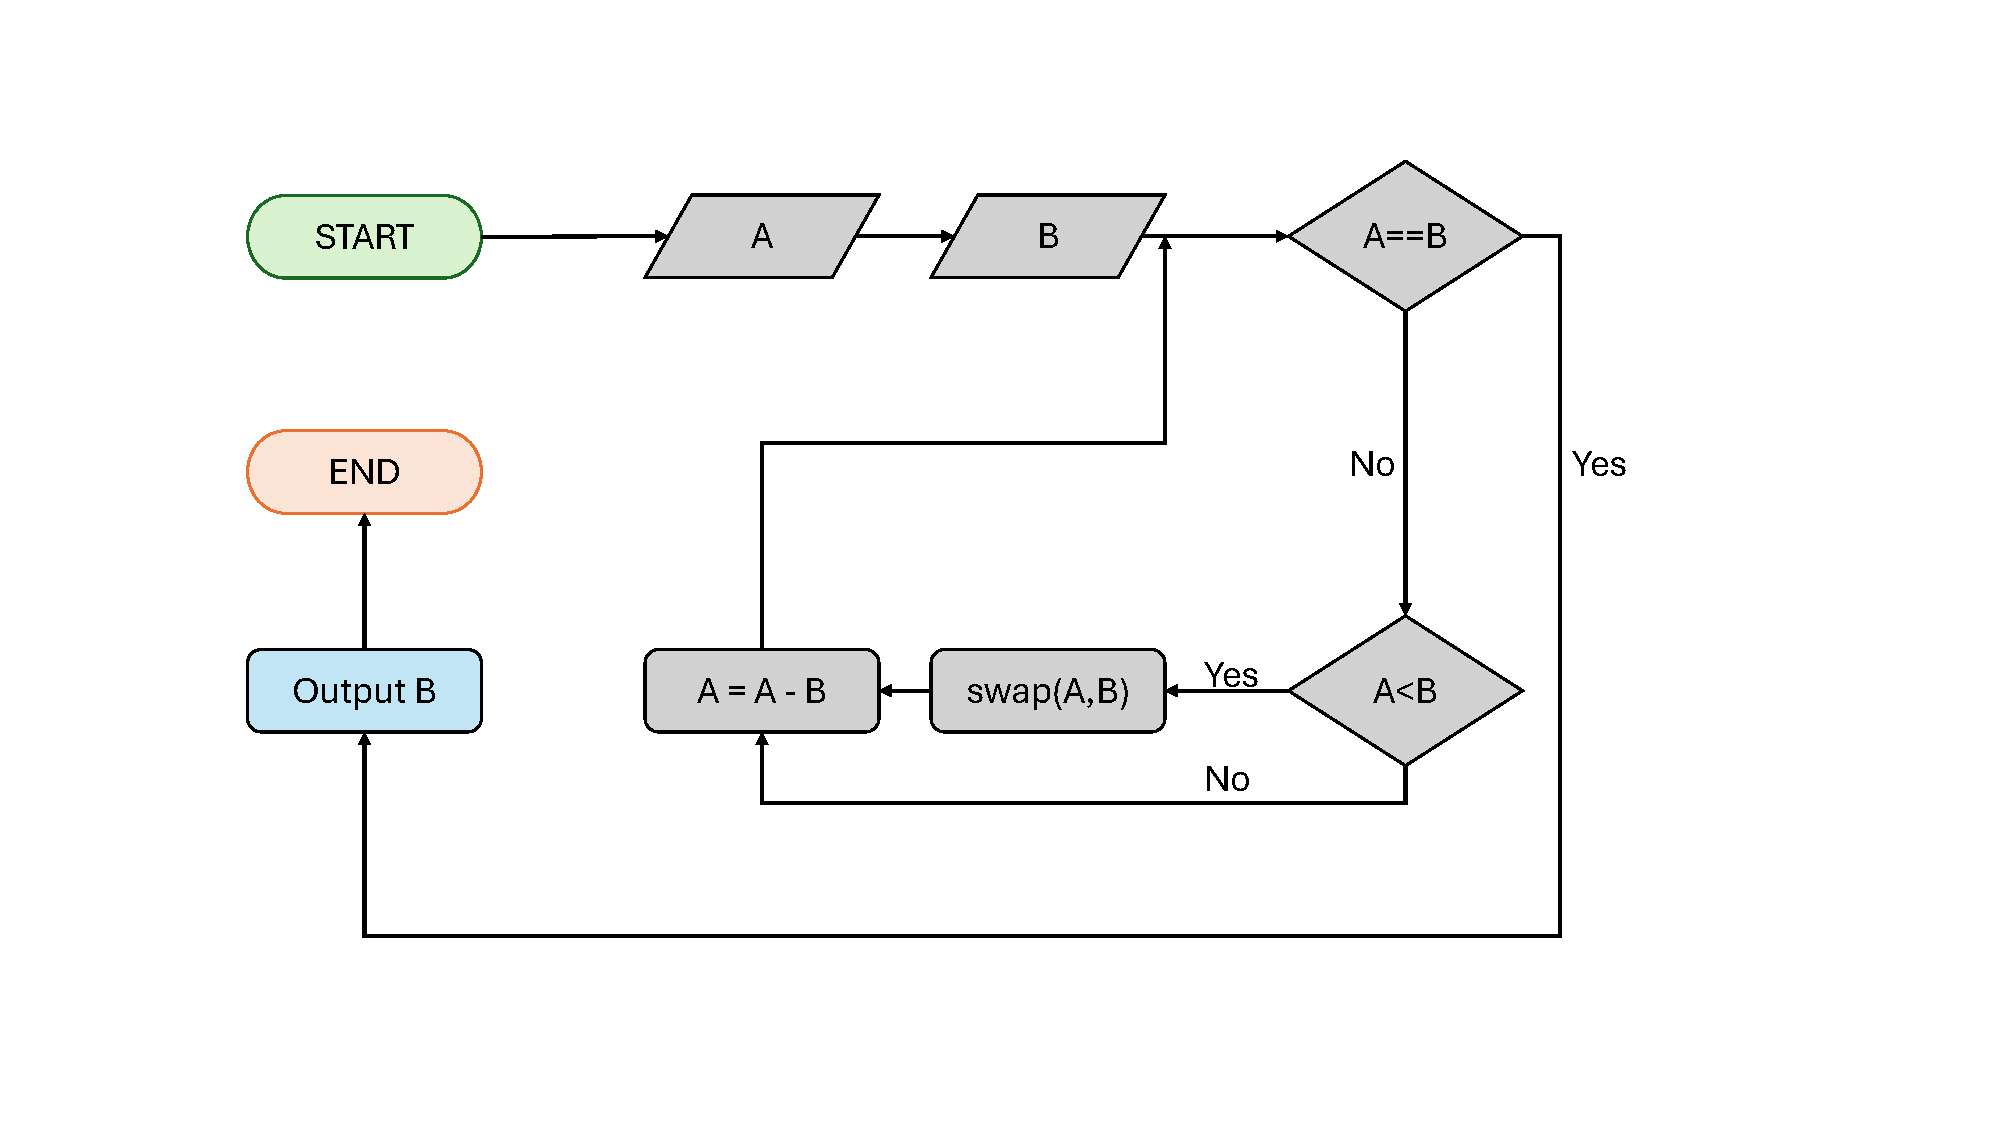
\includegraphics[width=\linewidth]{graphics/example.pdf}
  \caption{Example graphics.}
  \label{fig:example}
\end{figure}

Table stuff going in \Cref{tab:example} \lipsum[6]
\begin{table}
	\caption{Weird table title example.} 
	\label{tab:example}
	\begin{tabular}{lr}
		\toprule
		\multicolumn{2}{c}{Channel \hspace{2cm} Responses} \\ 
		\midrule
		DevOps Chat Slack & 3 \\ 
		Devops Weekly Newsletter & 24  \\ 
		Facebook & 3 \\ 
		LinkedIn & 7 \\ 
		\bottomrule
	\end{tabular}
\end{table}

Algorithm stuff can be written as in Algorithm \ref{alg:beaver_mult} \lipsum[6]

\begin{algorithm}
    \caption{Multiplication of secret shared values using Beaver's triple}
    \label{alg:beaver_mult}

    \textbf{\textsc{Input}}: $[x_1], [x_2]$ - secret shares of the inputs for multiplication
    \\
    \textbf{\textsc{Ouput}}: $[y]$ - secret share of the output, where $y=x_1x_2$
    \\
    \\
    \textbf{\textsc{Triple generation}}: Party $P_2$ (similar to a dealer) generates random $a,b$ values and $c$ such that $c=ab$. $P_2$ sends secret shares of $[a],[b],[c]$ to parties $P_0, P_1$.
    \\
    \\
    \textbf{\textsc{Multiplication}}: Each party evaluates:

    \begin{algorithmic}
         
        \State Compute $[\Delta a] = [x_1] - [a]$, $[\Delta b] = [x_2] - [b]$
        \State Exchange $[\Delta a], [\Delta b]$ with the other party and reconstruct $\Delta a, \Delta b$
        \State Evaluate $[w] = [c] + \Delta a [b] + \Delta b [a] + \Delta a \Delta b$
        \State return $[w]$
        
    \end{algorithmic}

\end{algorithm}

\section{This is a section of a chapter}
\label{sec:intro:section}

\lipsum[7]

\subsection{This is a subsection of a section}
\label{sec:intro:subsection}

\lipsum[8]

\subsubsection{This is a sub-subsection of a subsection}
\label{sec:intro:subsubsection}

\lipsum[9]